\subsection{Littlewood Principles and Lusin Approximation}

The measurable world is often controlled by ordinary topological objects after discarding a small exceptional set. In the real-line finite-measure setting, this principle has three recurring forms: measurable sets are nearly elementary, measurable functions are nearly continuous, and a.e. convergence is nearly uniform.

\begin{principle} \label{pr:littlewood-three-principles-finite-measure-real-line} \hlt{Littlewood's Three Principles, Finite-Measure Form}\\
For subsets of the real line with finite measure:
\begin{enumerate}[label=(\roman*)]
\setlength{\itemsep}{0pt}
\item measurable sets are nearly finite unions of intervals; see Corollary \ref{cor:real-line-finite-open-interval-approximation};
\item measurable functions are nearly continuous; this is Lusin's theorem below;
\item a.e. pointwise convergence is nearly uniform; see Egoroff's theorem, Theorem \ref{thm:egoroff-finite-measure}.
\end{enumerate}
\hlt{Key Insight}: The word ``nearly'' means after changing or discarding a set of arbitrarily small measure.
\end{principle}

\begin{lemma} \label{lem:real-line-continuous-extension-from-closed-set} \hlt{Continuous Extension from a Closed Subset of $\R$}\\
Let $F\subseteq\R$ be closed and let $h:F\to\R$ be continuous. Then there exists $g\in C(\R)$ such that $g|_F=h$.
\begin{proof} Cases $F=\emptyset$ and $F=\R$ are immediate. Otherwise $\R\setminus F=\bigsqcup_\alpha I_\alpha$, set $g=h$ on $F$; on each component:
\begin{enumerate}[label=(\roman*)]
\setlength{\itemsep}{0pt}
\item If $I_\alpha=(a,b)$, set $g(x)\defeq\frac{b-x}{b-a}h(a)+\frac{x-a}{b-a}h(b)$.
\item If $I_\alpha=(-\infty,b)$, set $g(x)\defeq h(b)$.
\item If $I_\alpha=(a,+\infty)$, set $g(x)\defeq h(a)$.
\end{enumerate}
The formulas give continuity off $F$; at $x\in F$, adjacent finite endpoints converge to $x$.\\
Hence continuity of $h$ gives $g(y)\to h(x)$ as $y\to x$. Thus $g\in C(\R)$ and $g|_F=h$.\\
\hlt{Structural Commentary}: Fill complementary intervals.\\
\hlt{Key Insight}: Interpolate between boundary values.
\end{proof}
\end{lemma}

\begin{proposition} \label{prop:simple-functions-continuous-on-large-closed-set} \hlt{Simple Functions Are Nearly Continuous}\\
Let $E\in\mathcal{L}^1$ with $m(E)<+\infty$, and $s:E\to\R$ measurable simple. $\forall \varepsilon>0$, $\exists F\subseteq E$ and $g:\R\to\R$ such that:
\begin{enumerate}[label=(\roman*)]
\setlength{\itemsep}{0pt}
\item $F$ is closed.
\item $g\in C(\R)$ and $g=s$ on $F$.
\item $m(E\setminus F)<\varepsilon$.
\end{enumerate}
\begin{proof} If $E=\emptyset$, take $F=\emptyset$ and $g=0$. Otherwise $s=\sum\limits_{i=1}^{N}a_i\mathbf{1}_{E_i}$ with disjoint measurable $E_i$ and $E=\bigsqcup_iE_i$. Choose closed $F_i\subseteq E_i$ with $m(E_i\setminus F_i)<\frac{\varepsilon}{N}$, set $F\defeq\bigcup_iF_i$, and define $h:F\to\R$ by $h|_{F_i}\defeq a_i$.
\begin{enumerate}[label=(\roman*)]
\setlength{\itemsep}{0pt}
\item Each $F_i$ is closed and $N<+\infty$, so $F$ is closed; also $F\subseteq E$.
\item For $x\in F_i$, the closed set $\bigcup_{j\neq i}F_j$ misses $x$, so $h$ is locally constant at $x$ in $F$; hence $h\in C(F)$.\\
Lemma \ref{lem:real-line-continuous-extension-from-closed-set} gives $g\in C(\R)$ with $g|_F=h=s|_F$.
\item $m(E\setminus F)\leq\sum_i m(E_i\setminus F_i)<\varepsilon$.
\end{enumerate}
\hlt{Structural Commentary}: Closed cores isolate simple levels.\\
\hlt{Key Insight}: Approximate each level set from inside, then extend.
\end{proof}
\end{proposition}

\begin{theorem} \label{thm:lusin-theorem-finite-measure-real-line} \hlt{Lusin's Theorem}\\
Let $E\in\mathcal{L}^1$ with $m(E)<+\infty$, $f:E\to\R$ measurable. $\forall \varepsilon>0$, $\exists F\subseteq E$ and $g:\R\to\R$ such that:
\begin{enumerate}[label=(\roman*)]
\setlength{\itemsep}{0pt}
\item $F$ is closed.
\item $g\in C(\R)$ and $g=f$ on $F$.
\item $m(E\setminus F)<\varepsilon$.
\end{enumerate}
\begin{proof} Take simple $s_n:E\to\R$ with $s_n\to f$ pointwise.\\
Pick $A\subseteq E$ with $s_n\to f$ uniformly on $A$ and $m(E\setminus A)<\frac{\varepsilon}{4}$, and closed $F_0\subseteq A$ with $m(A\setminus F_0)<\frac{\varepsilon}{4}$.\\
For $n\geq1$, choose closed $F_n\subseteq E$ with $s_n|_{F_n}\in C(F_n)$ and $m(E\setminus F_n)<\varepsilon2^{-(n+1)}$. Set $F\defeq\bigcap_{n\geq0}F_n$.
\begin{enumerate}[label=(\roman*)]
\setlength{\itemsep}{0pt}
\item $F$ is an intersection of closed sets and $F\subseteq E$.
\item Since $F\subseteq F_0\subseteq A$, the continuous functions $s_n|_F$ converge uniformly to $f|_F$, so $f|_F\in C(F)$.\\
Lemma \ref{lem:real-line-continuous-extension-from-closed-set} extends $f|_F$ to $g\in C(\R)$.
\item $m(E\setminus F)\leq m(E\setminus F_0)+\sum_{n\geq1}m(E\setminus F_n)<\varepsilon$.
\end{enumerate}
\hlt{Structural Commentary}: Discard a small set to gain continuity.\\
\hlt{Key Insight}: Simple cores plus Egoroff give uniform continuous limits.
\end{proof}
\end{theorem}

\begin{figure}[H]
  \centering
  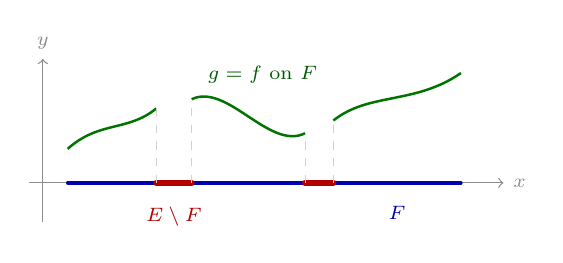
\begin{tikzpicture}[
  scale=0.9,
  every node/.style={font=\scriptsize},
  axis/.style={->, black!45, line width=0.45pt},
  core/.style={blue!70!black, line width=1.2pt, line cap=round},
  gap/.style={red!70!black, line width=2.2pt, line cap=round},
  curve/.style={draw=green!45!black, line width=0.9pt},
  guide/.style={draw=black!18, dashed, line width=0.35pt},
  note/.style={fill=white, inner sep=1pt}
]
  \draw[axis] (-3.35,0) -- (3.35,0) node[right] {$x$};
  \draw[axis] (-3.15,-0.55) -- (-3.15,1.75) node[above] {$y$};

  \draw[core] (-2.8,0) -- (-1.55,0);
  \draw[core] (-1.05,0) -- (0.55,0);
  \draw[core] (0.95,0) -- (2.75,0);

  \draw[gap] (-1.55,0) -- (-1.05,0);
  \draw[gap] (0.55,0) -- (0.95,0);
  \node[blue!70!black, below=5pt] at (1.85,0) {$F$};
  \node[red!70!black, below=5pt] at (-1.30,0) {$E\setminus F$};

  \draw[curve]
    (-2.8,0.48)
      .. controls (-2.35,0.88) and (-1.95,0.72) .. (-1.55,1.05);
  \draw[curve]
    (-1.05,1.18)
      .. controls (-0.55,1.42) and (0.05,0.45) .. (0.55,0.70);
  \draw[curve]
    (0.95,0.88)
      .. controls (1.45,1.28) and (2.10,1.10) .. (2.75,1.55);

  \draw[guide] (-1.55,0) -- (-1.55,1.05);
  \draw[guide] (-1.05,0) -- (-1.05,1.18);
  \draw[guide] (0.55,0) -- (0.55,0.70);
  \draw[guide] (0.95,0) -- (0.95,0.88);

  \node[green!35!black, note] at (-0.05,1.52) {$g=f$ on $F$};
\end{tikzpicture}

  \caption{Lusin's theorem: keep \textcolor{blue!70!black}{$F$}, discard \textcolor{red!70!black}{$E\setminus F$}, and extend with \textcolor{green!45!black}{$g=f$ on $F$}.}
  \label{fig:lusin-large-closed-set}
\end{figure}
